\scanpage{28}
\mspage{9}
équivaut à l'équation \deleted{\unsure{identique}} \deleted{\unsure{correspondante}} \inserted{\unsure{analogue}} en $\widetilde\alpha$
\[
(26)\qquad\widetilde\alpha\rho^{-1}(\unsure{\widehat\alpha|\widetilde\alpha})\rho^{-2}(\unsure{\widehat\alpha|\widetilde\alpha})=1,
\qquad\boxed{(27)\quad\widetilde\alpha=\eta^{-1}l_0^\gamma\varepsilon_0(\eta)}
\]
\deleted{$\unsure{\varepsilon}$}
Considérons maintenant le groupoïde \inserted{$\mathrm{III}_J$} induit par le groupoïde précédent \inserted{$\mathrm{II}_J$} sur l'ens des trois sommets $Q_i$, c'est aussi le groupoïde engendré par le graphe à trois sommets $Q_i$ $(i\in J)$ et six arcs orientés $\widetilde a_i^\omega$ et leurs opposés, avec les seules relations $(16)$ (ens de 6 relations stable par $G_J$, et se réduisant en fait à deux relations effectives\ldots).
\figure{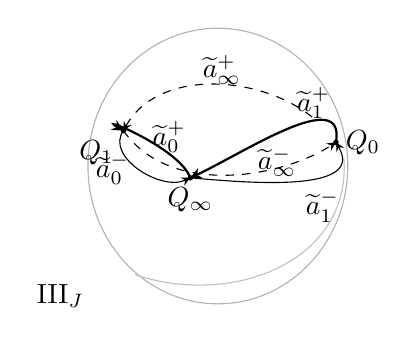
\begin{tikzpicture}[x=1cm,y=1cm,>=stealth]
\draw[gray!60] (0,.1) ellipse (1.65 and 1.75);
\draw[gray!50] (-1.05,-1.28) .. controls (.2,-1.7) and (1.7,-1.1) .. (1.6,.2);
\coordinate (A) at (-1.2,.55);\coordinate (B) at (-.35,-.05);\coordinate (C) at (1.5,.4);
\foreach \p in {A,B,C}{\fill(\p) circle(.035);}
\draw[->,thick] (B) to[out=110,in=150] node[right] {$\widetilde a_0^+$} (A);
\draw[->] (A) to[out=235,in=205] node[left] {$\widetilde a_0^-$} (B);
\draw[->,thick] (C) to[out=80,in=25] node[above right] {$\widetilde a_1^+$} (B);
\draw[->] (B) to[out=-5,in=300] node[below right] {$\widetilde a_1^-$} (C);
\draw[<-,dashed] (A) .. controls (-.75,1.35) and (.55,1.25) .. (1.2,.72);
\node at(.05,1.32){$\widetilde a_\infty^+$};
\draw[->,dashed] (A) .. controls (-.6,-.3) and (.8,-.05) .. (C);
\node at(.75,.15){$\widetilde a_\infty^-$};
\node[below left] at(A){$Q_1$};\node[below] at(B){$Q_\infty$};\node[right] at(C){$Q_0$};
\node at(-2,-1.55){$\mathrm{III}_J$};
\end{tikzpicture}}
Le groupe $\{1,\tau\}$ y opère dans le graphe avec relations, par
\[
(27)\qquad\tau Q_i=Q_i,\quad\tau\widetilde a_i^\omega=(\widetilde a_i^{\omega'})^{-1}
\]
La donnée d'un \deleted{\unsure{autom.}} \inserted{endom.} du groupoïde $\widehat{\mathrm{III}}_J$, fixant les sommets et commutant à $G_J$, équivaut à \unsure{celle} d'un $\widetilde\alpha\in\widehat\Pi_{0,3}$, \deleted{$\unsure{\in\widehat{\mathbb Z}}$}, satisfaisant \deleted{\unsure{l'équation rel.}} $(26)$. On aura, en introduisant
\[
(28)\qquad\widetilde\lambda_i^\omega=\widetilde a_i^{\omega'}\widetilde a_i^\omega\in\deleted{\unsure{Q_{\omega'i}}}\inserted{\pi(Q_{\omega'i})}
\]
(\unsure{comparer à la définition dans le groupoïde} $\mathrm{II}_J$ ! $\lambda_i^\omega=a_i^{\omega'}a_i^\omega$)
\diagram{\begin{tikzcd}[ampersand replacement=\&,column sep=small]
Q_{\omega i}\arrow[rrr,bend right=45,"\widetilde a_i^{\omega'}"']\&R_i^{\omega'}\arrow[l,dashed,no head]\arrow[r,dashed,bend right=40]\&R_i^\omega\arrow[l,dashed,bend right=40,"a_i^\omega"']\arrow[r,dashed,no head]\&Q_{\omega'i}\arrow[lll,bend right=45,"\widetilde a_i^{\unsure{\omega}}"']
\end{tikzcd}}
\margin{\deleted{il semblerait raisonnable de changer les notations $\widetilde a_i^\omega$ devenant $\widetilde a_i^{\omega'}$ \unsure{au-dessous}.}\quad $*$ \unsure{obtenir}, \unsure{une définition des} $\psi_i^\alpha$ \unsure{qui} \unsure{donne} dans $(29)$ \unsure{ainsi}. \unsure{cf.} \unsure{voir} plus bas}
\[
(29)\qquad u(\widetilde\lambda_i^\omega)=\overset{*}{\psi_{\omega'i}^{\omega'}}(\widetilde\alpha\varepsilon_0(\widetilde\alpha))\widetilde\lambda_i^\omega
=\psi_{\omega'i}^{\omega'}(\widetilde\alpha\varepsilon_0(\widetilde\alpha)l_0)
\]
Dans le cas où $\widetilde\alpha$ provient de $\eta,\gamma$ par $(27)$, on aura
\[
(\unsure{30})\qquad\widetilde\alpha\varepsilon_0(\widetilde\alpha)l_0=\eta^{-1}l_0^p\eta\qquad(p=2\gamma+1)\ ;
\]
\margin{27}
